Pour une présentation succinctes de quelques possibilités de \LaTeX{}
on peut faire un tour sur la page  \url{http://www.latextemplates.com/}
qui présente déjà un bon panorama.


%%%%%%%%%%%%%%%%%%%%%%%%%%%%%%%%%%%%%%%%%%%%%%%%%%%%%%%%%%%%%%%%%%%%%%%%%%%%%%%%%%%%%%%%%%%%%%%%%%%%%%%%%
\section{Logiciels}
%%%%%%%%%%%%%%%%%%%%%%%%%%%%%%%%%%%%%%%%%%%%%%%%%%%%%%%%%%%%%%%%%%%%%%%%%%%%%%%%%%%%%%%%%%%%%%%%%%%%%%%%%

Tout d'abord, il faut disposer d'un éditeur de texte et d'un compilateur.

\begin{itemize}
\item Sous Mac : installer MacTex  (éditeur + compilateur). L'éditeur s'appelle Texshop.  
\item Sous Linux : \LaTeX{} est installé de base, il vous faut juste un bon éditeur. Kile est très bien et suffisant
dans un premier temps. Les experts pourront utiliser Vim ou emacs. 
\item Sous Windows : installer Miktex d'abord (chercher avec un moteur de recherche) puis Texniccenter 
ou  Winshell par exemple.
\end{itemize}


\section{Format de fichiers et compilation}
En \LaTeX{}, on écrit un code ``barbare'' qui sera compil\'e par un programme. Sur vos terminaux c'est Kile 
qui compilera : il faut aller dans l'onglet ``\textbf{build}'' ou ``\textbf{construire}'', puis cliquer 
sur ``\textbf{compile}''. On choisit alors le type de compilation (Latex, pdfLatex, bibtex pour la
 bibliographie \ldots). 
\begin{itemize}
 \item si en sortie on veut un fichier ps : il faut faire ``\textbf{tex to dvi}'' puis  ``\textbf{dvi to ps}''
 \item si en sortie on veut un fichier pdf : il faut faire ``\textbf{pdfLatex}'' (mieux pour afficher des documents 
avec des hyperliens et des images de formats standards).
\end{itemize}



Le fichier \LaTeX{} du document que vous êtes en train de lire est  disponible ici : 
\href{http://josephsalmon.eu/enseignement/M1/introlatex.tex}{ceci est un lien hypertexte}.  
Son extension est  .tex. Une fois le fichier compilé,  on obtiendra un ``joli'' document en format .pdf 
ou bien .ps. Pour visualiser le résultat il suffit d'aller dans l'onglet  ``\textbf{build}'' 
(ou constuire), choisir ``\textbf{view}`` (ou voir) puis de sélectionner ``\textbf{Viewpdf}'' 
(si l'on a fait pdfLatex).\medskip

Ceci fait, on choisit la classe de document  que l'on veut créer.  Pour les projets,  
la classe ``\textbf{article}'' est recommandée (les plus motivés qui voudraient écrire un 
livre entier pourront utiliser la classe ``\textbf{book}''). Le document commence donc par la 
commande :\medskip

\begin{lstlisting}
\documentclass[a4paper,12pt]{article}
\end{lstlisting}

Les options d'une fonction \LaTeX{} sont toujours entre crochets. Ici elles déterminent le format 
(A4) du document, et définissent la taille par d\'efaut de la police (12pt).

\section{Les packages}

En dessous du choix de la classe on donne la définition des packages dont on a besoin. 
Les packages sont des bibliothèques utilisées pour des fonctions avancées, que l'on doit charger.
 Par exemple la commande  \lstinline+\usepackage{amsmath}+ charge le package ``\textbf{asmath}'',
 qui est utile  pour écrire des symboles mathématiques. Le package ``\textbf{babel}''  est lui 
utilisé pour écrire des accents (du moins avec l'option ``\textbf{french}''). En effet, les anglophones
 n'en ont pas besoin, donc initialement \LaTeX{} ne gère pas les accents. 
% L'intérêt du package est
%  donc de pallier ce manque. \medskip

Les packages sont des fichiers au format .sty. Ils sont pour la plupart déjà installés sur votre 
ordinateur (par Miktex ou Texshop). Par contre, il se peut que certains packages ne soient pas 
disponibles.  Pour les rendre utilisables pour la compilation il suffit de télécharger le fichier 
``\textbf{*.sty}''  sur internet (\eg sur le site du  \href{http://www.ctan.org/}{CTAN})
  et de le placer dans le dossier où vous éditez votre fichier .tex.

\section{Formules mathématiques et théorèmes}
On peut définir des environnements comme des théorèmes, des propositions, etc., avec:\medskip
\begin{lstlisting}
\newtheorem{theorem}{Theorem}[section] 
\newtheorem{prop}[theorem]{Proposition}
\end{lstlisting}
Cela donne :

\begin{theorem}
 L'ensemble des nombres premiers est infini.
\end{theorem}
Les théorèmes  sont ainsi numérotés par \LaTeX{} de manière automatique.

\begin{theorem}
 L'ensemble des nombres premiers congrus à 1 modulo 4 est infini.
\end{theorem}

\begin{proof}
 ici on ferait la démonstration ... mais  je vous la laisse en exercice.
\end{proof}

Une fois les packages définis, on peut créer des raccourcis pour les quantités qui reviennent 
souvent ou des fonctions. Par exemple, on peut définir un raccourcis pour la commande qui créée une 
fonction: \lstinline+\newcommand{\nc}{\newcommand}+.

\begin{rem}
 Toutes les fonctions (au sens informatique du terme) connues par \LaTeX{} commencent par $\backslash$ 
(backslash) comme par exemple \lstinline+\sum+
 qui permet d'afficher le symbole de sommation $\sum_{i=1}^{4}$. 
\end{rem}


Pour les formules mathématiques, on doit les placer entre deux signes 
$\$$ pour qu'elles soit interprétées comme des commandes spéciales et non comme du texte. 
Ainsi, pour écrire le signe de sommation ci-dessus on écrit \lstinline+$\sum\_{i=1}^{4}$+ dans le 
fichier .tex. Si l'on veut afficher des calculs sur une ligne à part on peut par exemple écrire 
\[\mathcal{S}f = \sum_{k\in\mathbb{Z}} \hat{f}[k] e^{i2\pi kt/T}, \] 
en mettant cette fois les formules  entre  les commandes 
\lstinline+\[+ et \lstinline+\]+. Il est en fait recommandé d'utiliser un environnement qui commence par la 
commande 
\lstinline+\begin{blabla}+ et finit par la commande \lstinline+\end{blabla}+ pour ce genre de ligne de calcul.
Pensez plut\^ot \`a utiliser \lstinline+\begin{equation}+, voir \lstinline+\begin{align}+ 
si l'on veut des calculs facilement:
\begin{align}
 \mathcal{S}f & = \sum_{k\in\mathbb{Z}} \hat f[k] e^{i2\pi kt/T} \label{nomformule}\\
  & = \sum_{k\in\mathbb{Z}} \hat f[k] e^{i2\pi kt/T}
\end{align}

\begin{rem}
On notera que la numérotation s'est déclenchée toute seule pour les formules. 
On peut  leur donner des noms avec la commande \lstinline+label+,  dont la syntaxe est  \lstinline+\label{nomformule}+.  
On s'y réfère plus tard dans le document avec \lstinline+\ref{nomformule}+ (ou \lstinline+\eqref{nomformule}+), ce qui affiche
le num\'ero \ref{nomformule} (respectivement \eqref{nomformule}). 
Ainsi l'ordre des équations peut être changé sans avoir besoin de re-numéroter tout un document. 
Si l'on ne veut pas numéroter une équation,  on met une étoile à la fin de l'environnement 
(écrire \lstinline+align*+ à la place d'\lstinline+align+ par exemple).
\end{rem}



Pour un grand panel de symboles mathématiques, il suffit de regarder les raccourcis fournis par l'éditeur 
que vous utilisez ou de chercher sur Internet un lexique. Voici néanmoins quelques commandes : 
pour aller à la ligne  \lstinline+\\+, 
pour une nouvelle feuille \lstinline+\newpage+, pour les trois points  \lstinline+\ldots+.

On renvoit à \href{http://www.tex.ac.uk/tex-archive/info/symbols/comprehensive/symbols-a4.pdf}
{``The Comprehensive \LaTeX{} Symbol List''} par Scott Pakin pour une liste exhaustive de tous les
 symboles connus.


%%%%%%%%%%%%%%%%%%%%%%%%%%%%%%%%%%%%%%%%%%%%%%%%%%%%%%%%%%%%%%%%%%%%%%%%%%%%%%%%%%%%%%%%%%%%%%%%%%%%%%%%%
\section{Organisation du document}
%%%%%%%%%%%%%%%%%%%%%%%%%%%%%%%%%%%%%%%%%%%%%%%%%%%%%%%%%%%%%%%%%%%%%%%%%%%%%%%%%%%%%%%%%%%%%%%%%%%%%%%%%


On commence par donner un titre au  fichier, le nom de l'auteur et éventuellement la date par les
 commandes suivantes :\medskip

\begin{lstlisting}
\title{Faire un rapport en \LaTeX{}} 
\author{Nom} 
\date{}
\end{lstlisting}



Ensuite on commence le corps du document avec \lstinline+\begin{document}+ 
(ne pas oublier de fermer tout en bas par \lstinline+\end{document}+). 
On insère le titre avec \lstinline+\maketitle+ et la table des matières avec \lstinline+\tableofcontents+.
La construction de la table des matières se fait automatiquement. 
Elle donne l'arborescence du document, dans l'ordre où les chapitres et sous chapitres sont donnés 
dans le fichier .tex.\medskip	


On crée  des chapitres (resp. des sous chapitres) en écrivant au début d'un chapitre 
\lstinline+\chapter{le_nom_du_chapitre}+ 
(resp. \lstinline+\section{le_nom_du_sous-chapitre}+).  
\LaTeX{} numérote tout seul les chapitres dans l'ordre où ils se présentent. 
Si l'on intervertit deux chapitres, à la prochaine compilation les numéros seront automatiquement 
échangés. Attention, il faut parfois deux compilations pour afficher correctement la table des matières.  \medskip
 
Ceci fait, vous pouvez déjà commencer à rédiger un premier document, visuellement correcte avec
toutes les formules de mathématiques dont vous avez besoin. Au chapitre suivant on va voir 
quelques raffinements possibles pour égayer vos documents.



%%%%%%%%%%%%%%%%%%%%%%%%%%%%%%%%%%%%%%%%%%%%%%%%%%%%%%%%%%%%%%%%%%%%%%%%%%%%%%%%%%%%%%%%%%%%%%%%%%%%%%%%%
\section{Insérer une image }
%%%%%%%%%%%%%%%%%%%%%%%%%%%%%%%%%%%%%%%%%%%%%%%%%%%%%%%%%%%%%%%%%%%%%%%%%%%%%%%%%%%%%%%%%%%%%%%%%%%%%%%%%

Après avoir créé des graphiques avec \lstinline+R+, Python, ou Matlab, etc.,  vous pouvez avoir 
envie de les insérer dans votre rapport. Cette opération est plus compliquée qu'avec un éditeur 
de texte classique. Voici le code pour insérer l'image ci-dessous : \medskip
\begin{lstlisting}
\begin{figure}[htb]
\begin{minipage}[b]{0.33\linewidth}
  \centering
 \centerline{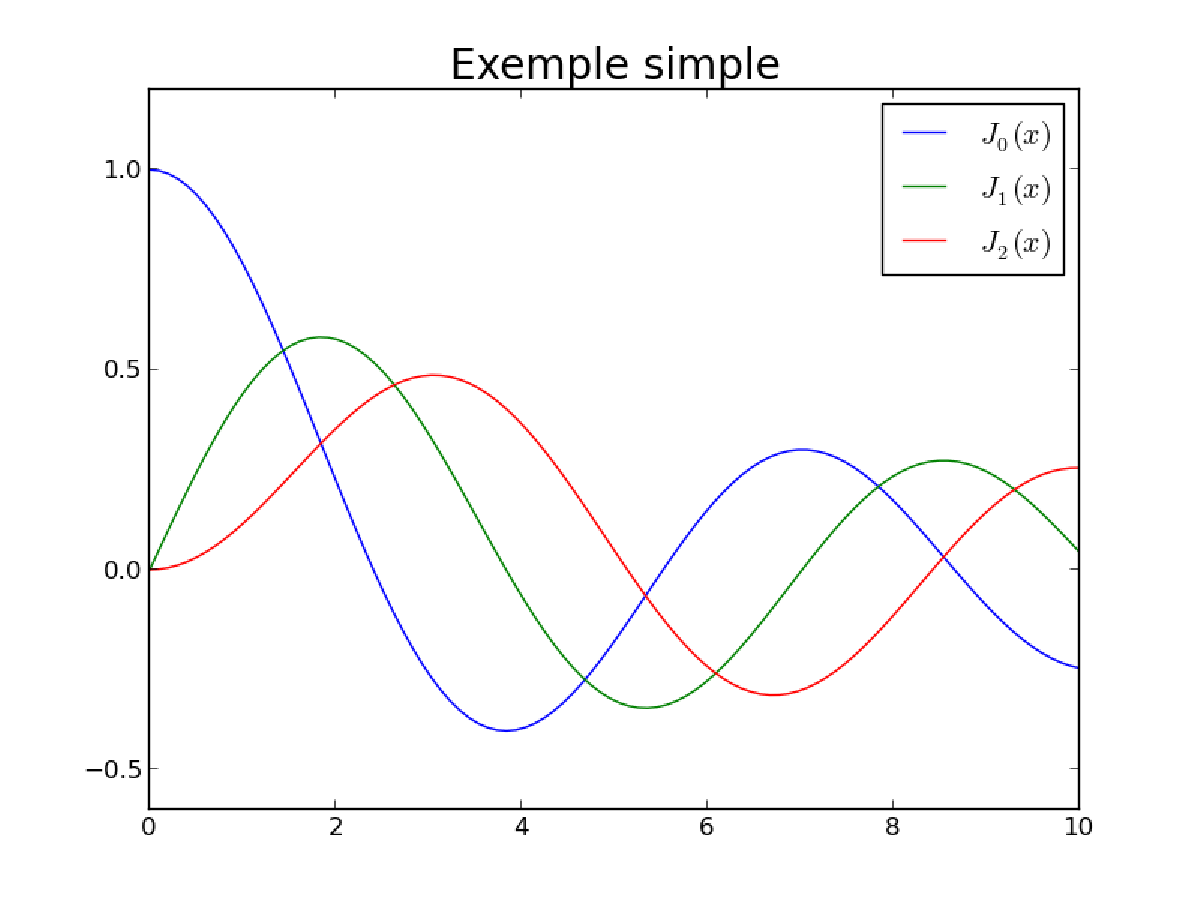
\includegraphics[clip,viewport=400 300 520 450,
width=1.\textwidth]{example_simple_png}}
  \vspace{0.1cm}
  \centerline{(A) version .png}\medskip
\end{minipage}
\hfill
\begin{minipage}[b]{.33\linewidth}
  \centering
 \centerline{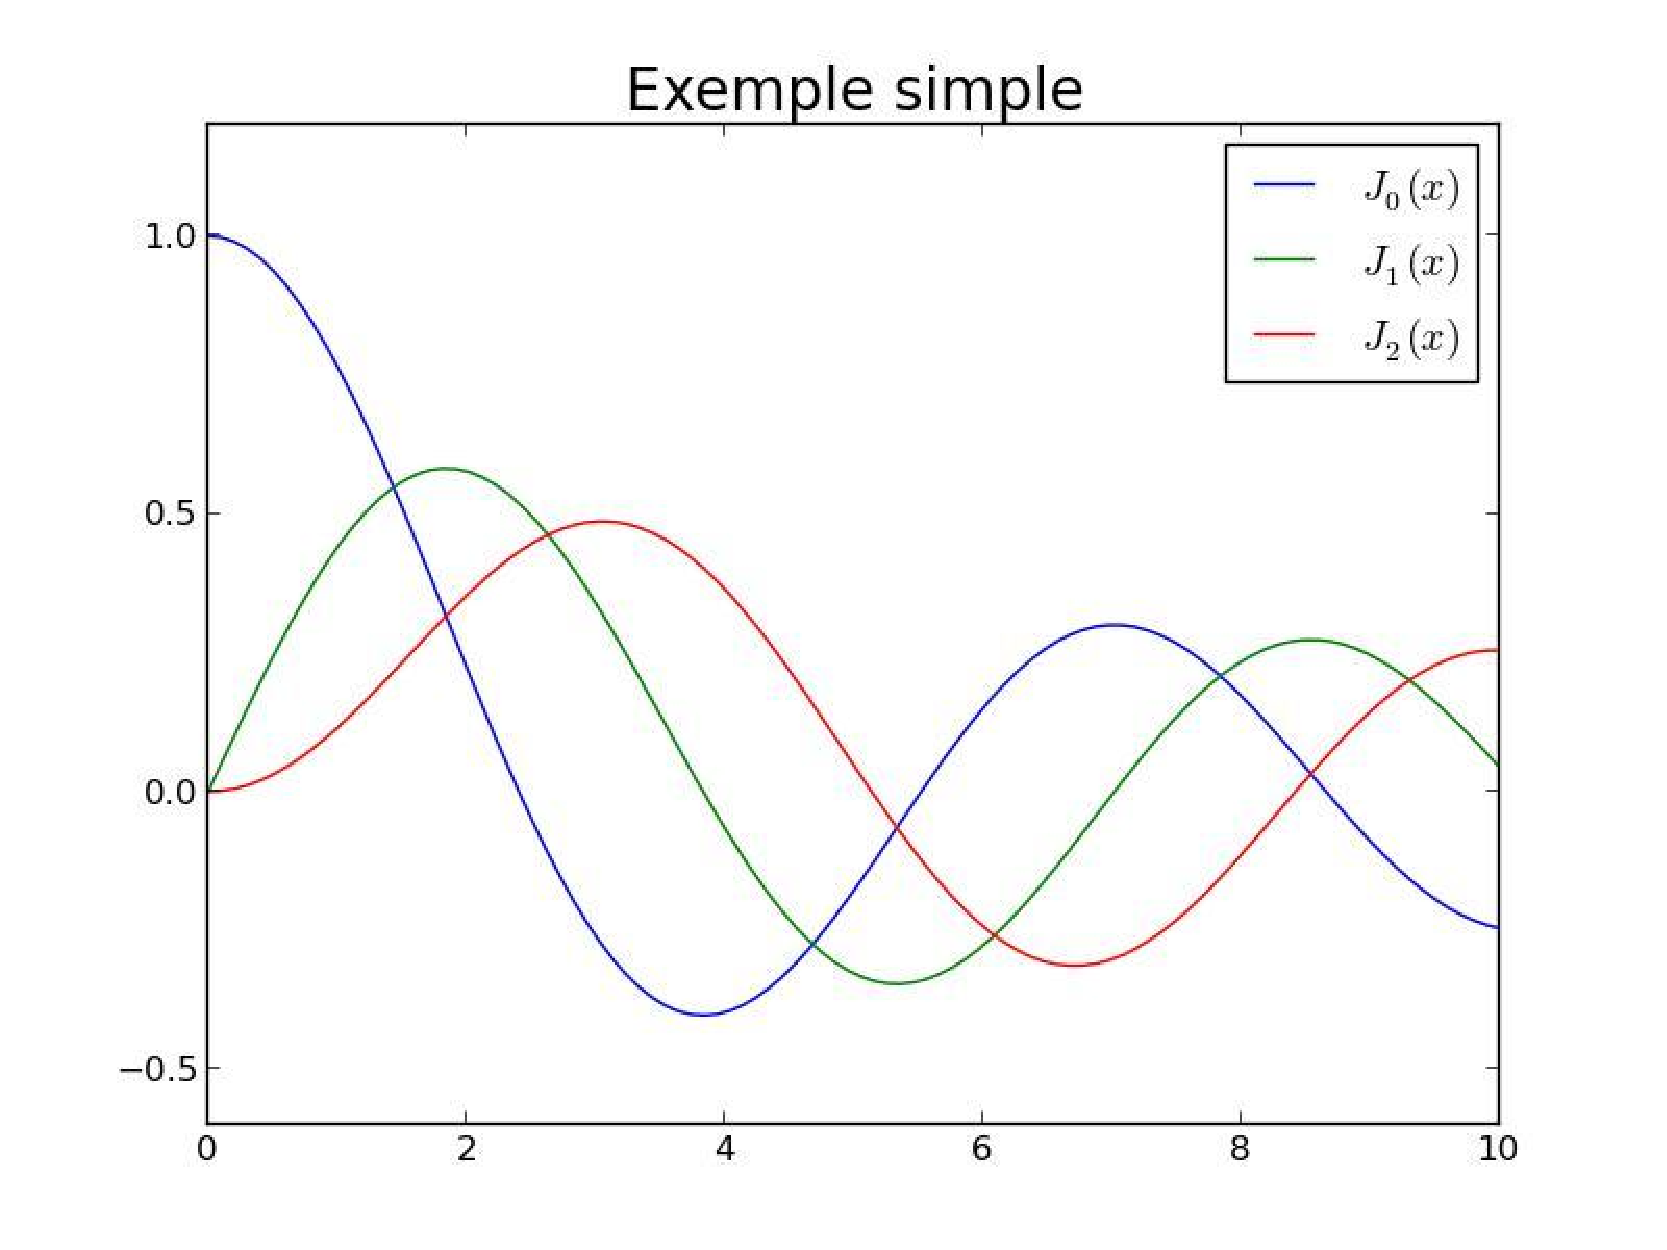
\includegraphics[clip=true,
 viewport=550 410 729 590,width=1.\textwidth]{example_simple_jpg}}
  \vspace{0.1cm}
  \centerline{(B) version .jpg}\medskip
\end{minipage}%
\hfill
\begin{minipage}[b]{.33\linewidth}
  \centering
 \centerline{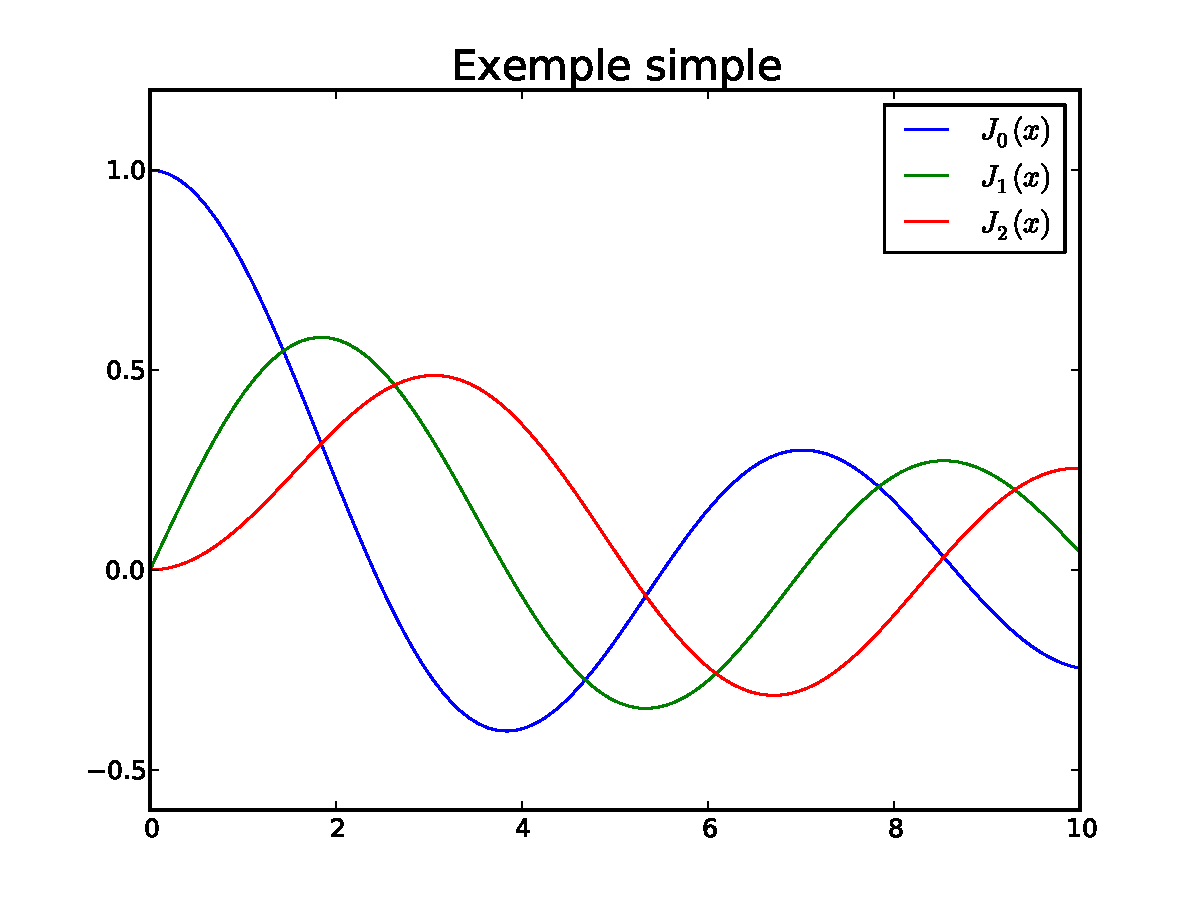
\includegraphics[clip,viewport=400 300 520 450,
 width=1.\textwidth]{example_simple_pdf}}
  \vspace{0.1cm}
  \centerline{(C) version .pdf}\medskip
\end{minipage}%
\caption{De pr\`es le .jpg c'est \textbf{VRAIMENT} nul}
\label{fig:ma_figure_zoom}
\end{figure}
\end{lstlisting} 

\begin{figure}[h]
\begin{minipage}[b]{0.33\linewidth}
  \centering
 \centerline{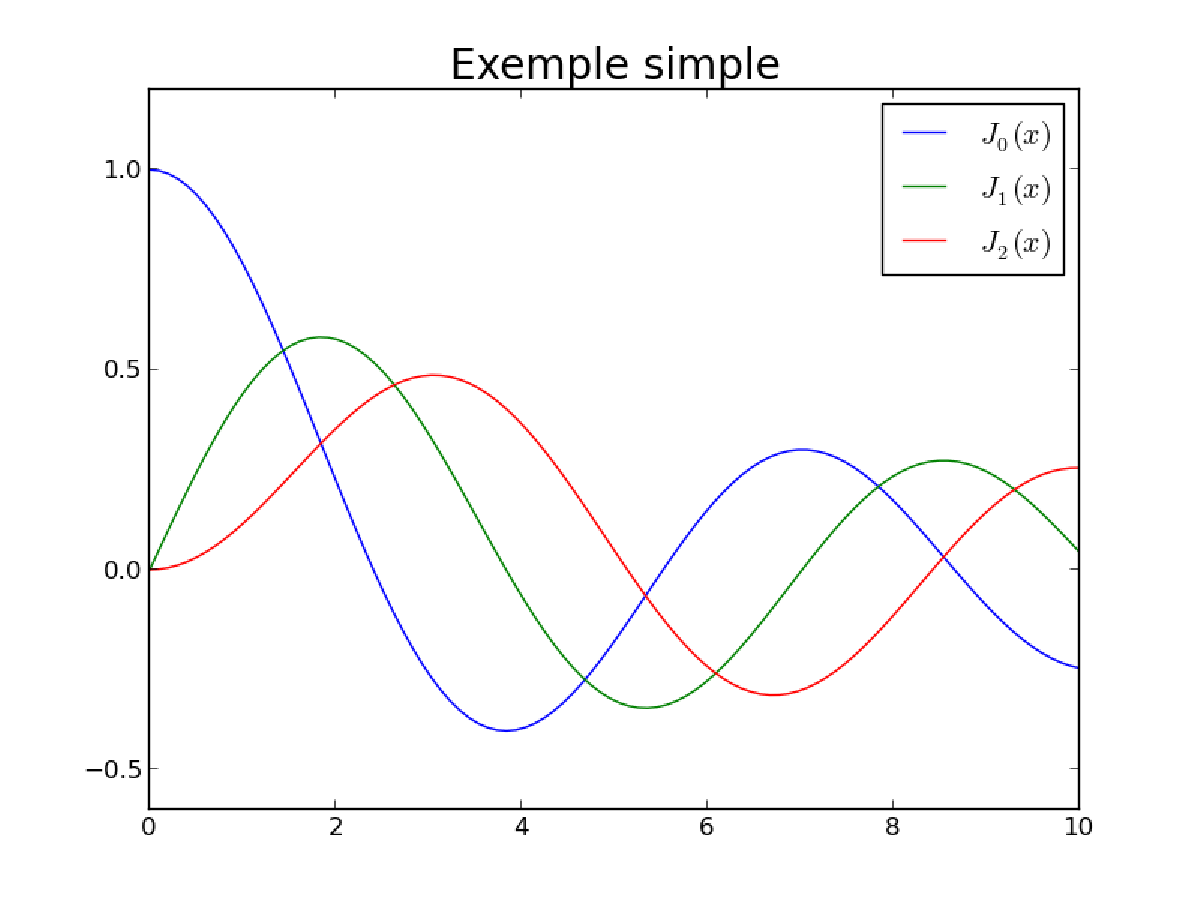
\includegraphics[width=1.\textwidth]{example_simple_png}}
  \vspace{0.1cm}
  \centerline{(A) Version .png}\medskip
\end{minipage}
\hfill
\begin{minipage}[b]{.33\linewidth}
  \centering
 \centerline{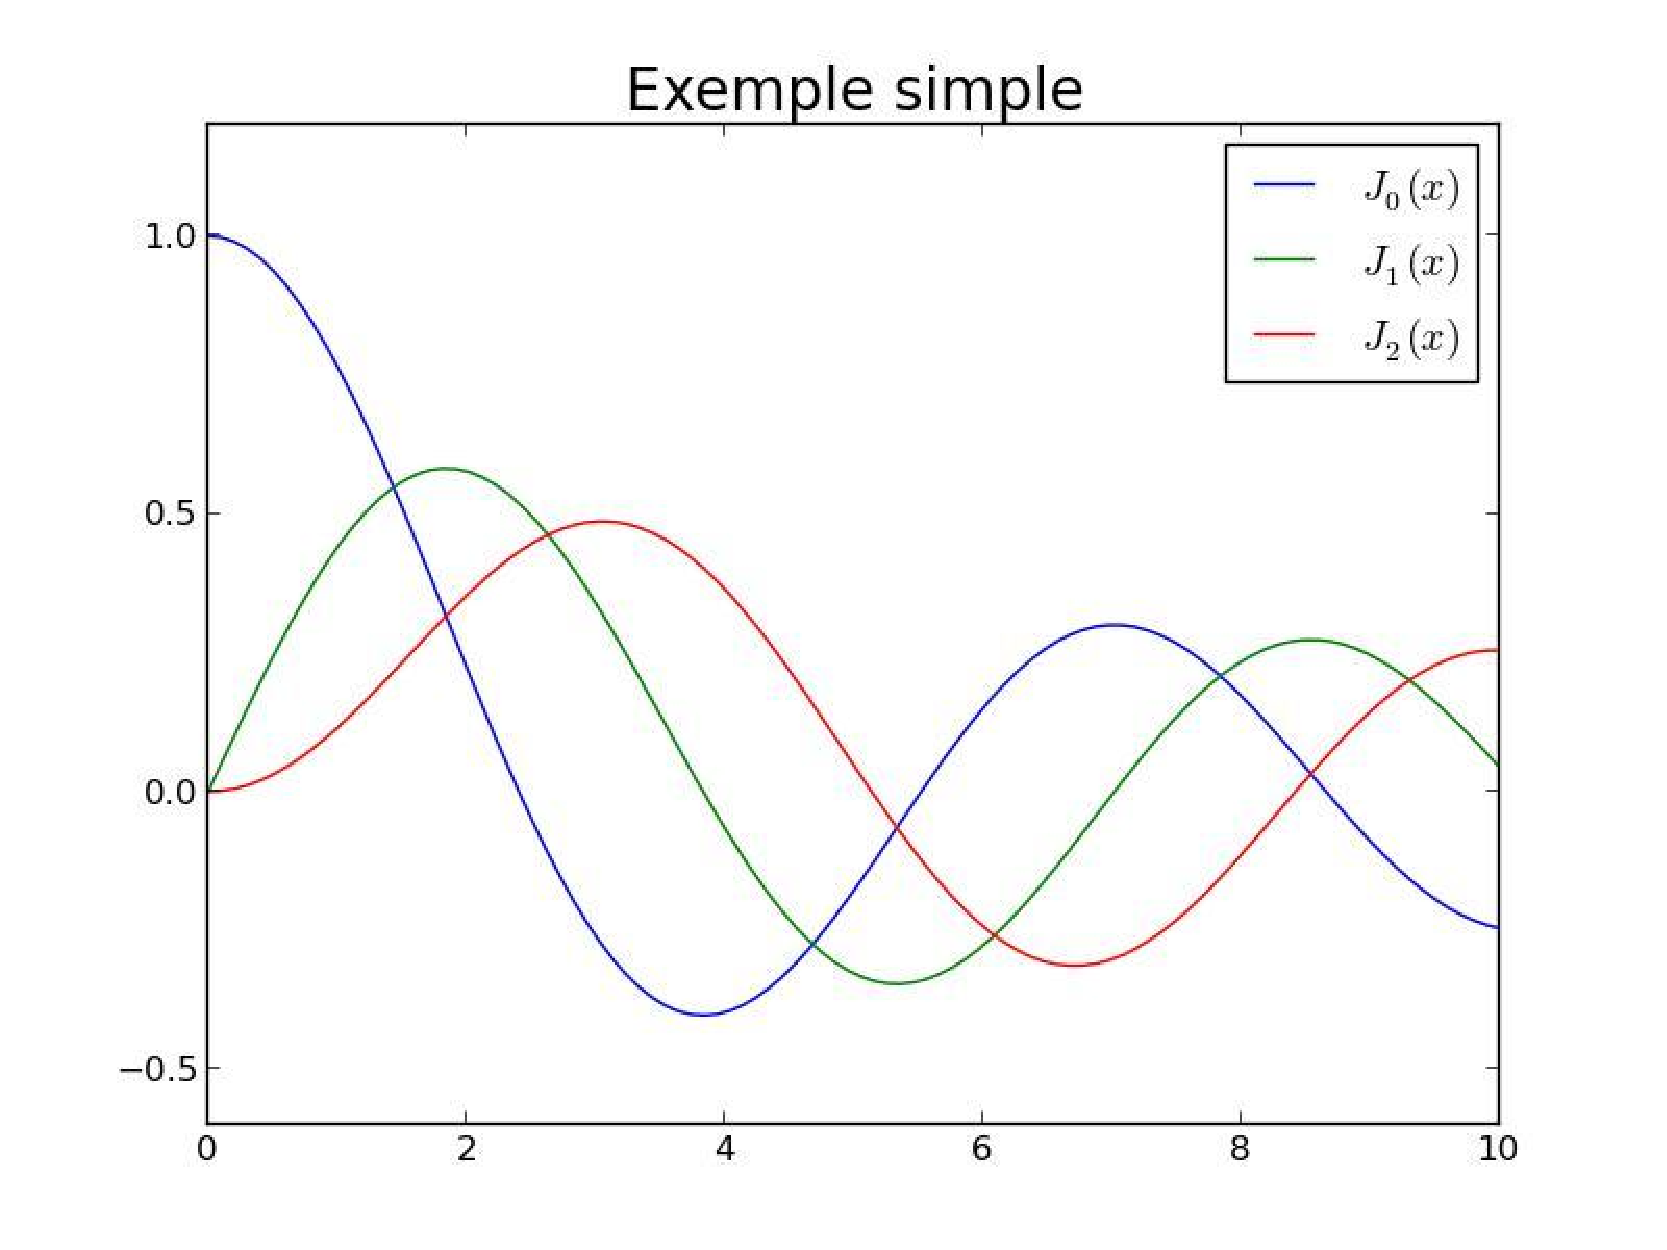
\includegraphics[width=1.\textwidth]{example_simple_jpg}}
  \vspace{0.1cm}
  \centerline{(B) Version .jpg}\medskip
\end{minipage}%
\hfill
\begin{minipage}[b]{.33\linewidth}
  \centering
 \centerline{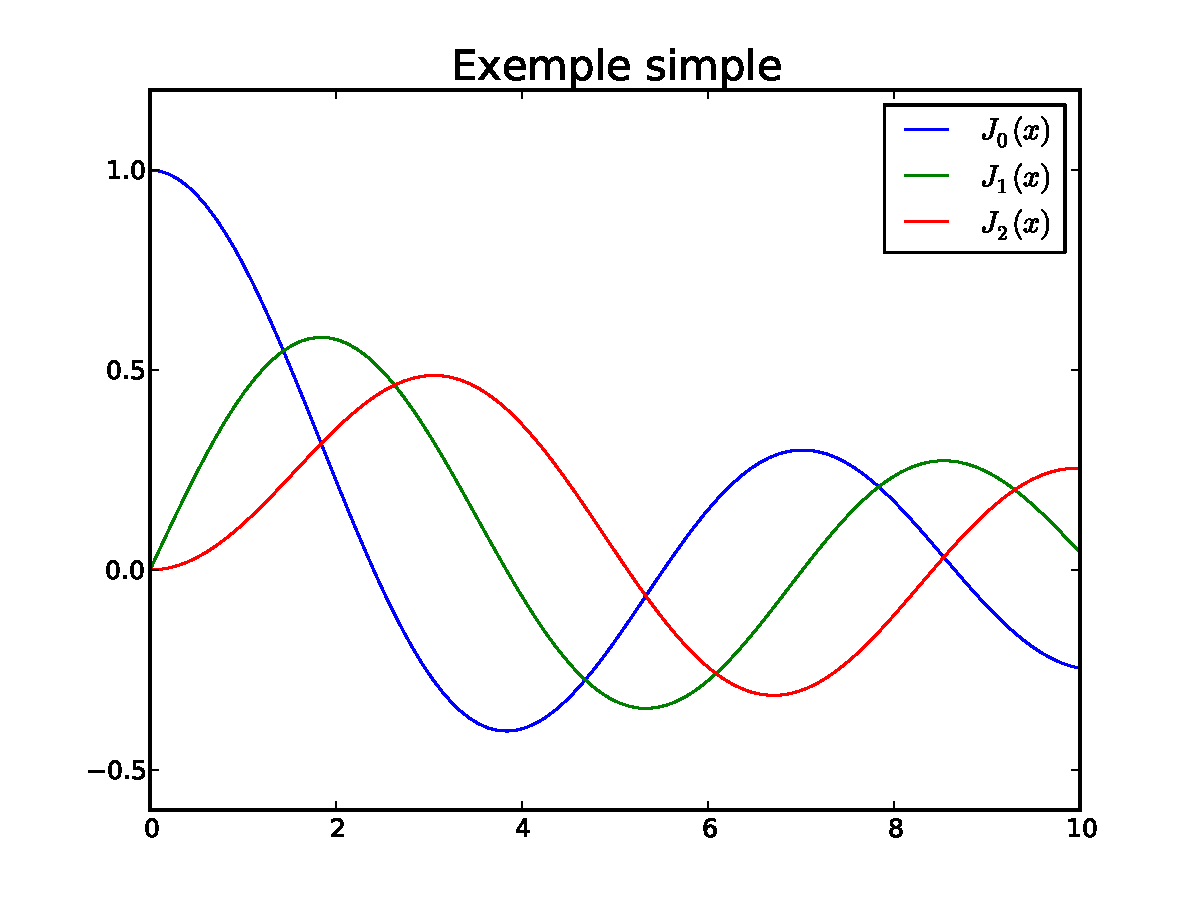
\includegraphics[width=1.\textwidth]{example_simple_pdf}}
  \vspace{0.1cm}
  \centerline{(C) version .pdf}\medskip
\end{minipage}%
\caption{De loin les trois formats se ressemblent...mais quand m\^eme le .jpg c'est bien nul}
\label{fig:ma_figure}
\end{figure}
L'image insérée doit se trouver par défaut dans le même répertoire où se trouve le fichier .tex 
que vous écrivez. On peut d\'eclarer \`a la main les sous dossiers, ou bien cr\'eer une fois
pour toute un dossier \lstinline+images+ et d\'eclarer son chemin d'acc\`es dans le préambule
avec
\begin{lstlisting}
\graphicspath{{images/}} 
\end{lstlisting}

% On pourra faire varier les paramètres de taille pour voir comment jouer sur la 
% taille de l'image que l'on insère. 
Il existe d'autres façons d'insérer des images, mais celle-ci à l'avantage de fonctionner~\ldots


En utilisant ''\textbf{pdfLatex}'' (largement conseillé)  on peut insérer des images au format .jpg, .png, 
.pdf, etc. En revanche, si l'on compile pour obtenir un fichier .ps avec ``\textbf{Latex}'' il 
faut insérer des images sous le format .eps. Les commandes en revanche ne diffèrent
 pas.

Grâce au label utilisé pour la figure, on peut se référer à celle-ci comme pour les équations,
 par la commande \lstinline+\ref{fig:ma_figure}+. Ainsi la première figure est la figure \ref{fig:ma_figure}.

Pour des documents visuellement agr\'eable utilisez les extensions .pdf et .eps, et surtout proscrire le .jpg!
notamment pour des graphiques ou des croquis. Pour les images photos, on pourra utiliser le .png qui lui aussi
\'evite les artefacts de compression du format .jpg .

\begin{figure}[htb]
\begin{minipage}[b]{0.33\linewidth}
  \centering
 \centerline{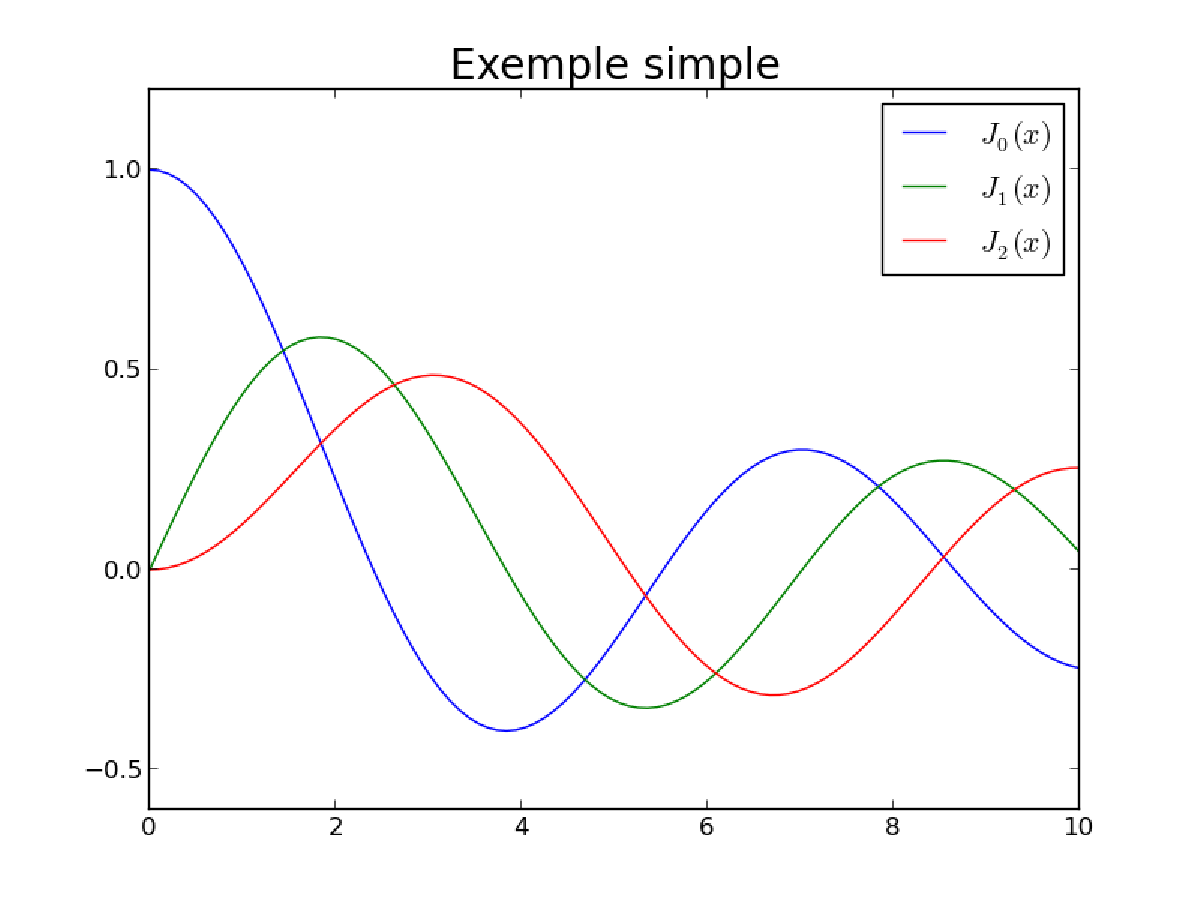
\includegraphics[clip,viewport=400 300 520 450,width=1.\textwidth]{example_simple_png}}
  \vspace{0.1cm}
  \centerline{(A) version .png}\medskip
\end{minipage}
\hfill
\begin{minipage}[b]{.33\linewidth}
  \centering
 \centerline{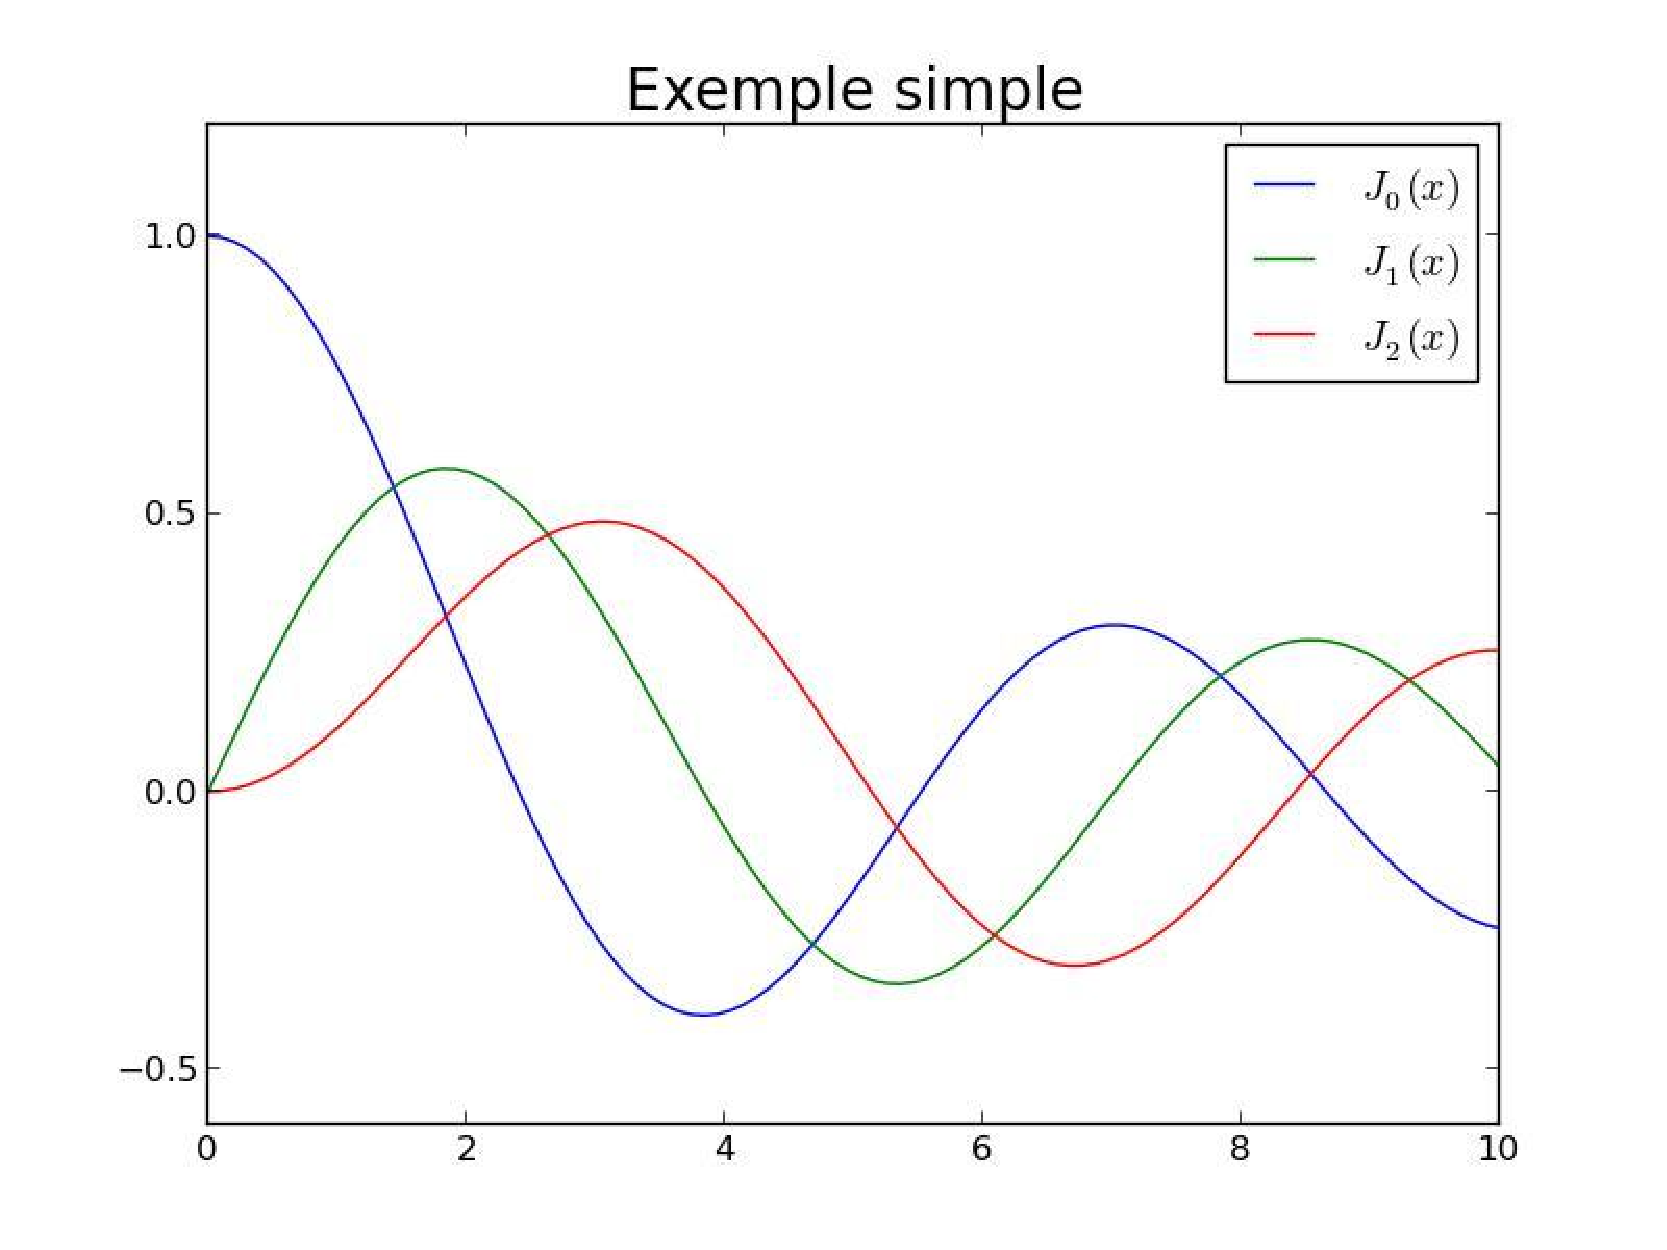
\includegraphics[clip=true,viewport=550 410 727 590,width=1.\textwidth]{example_simple_jpg}}
  \vspace{0.1cm}
  \centerline{(B) version .jpg}\medskip
\end{minipage}%
\hfill
\begin{minipage}[b]{.33\linewidth}
  \centering
 \centerline{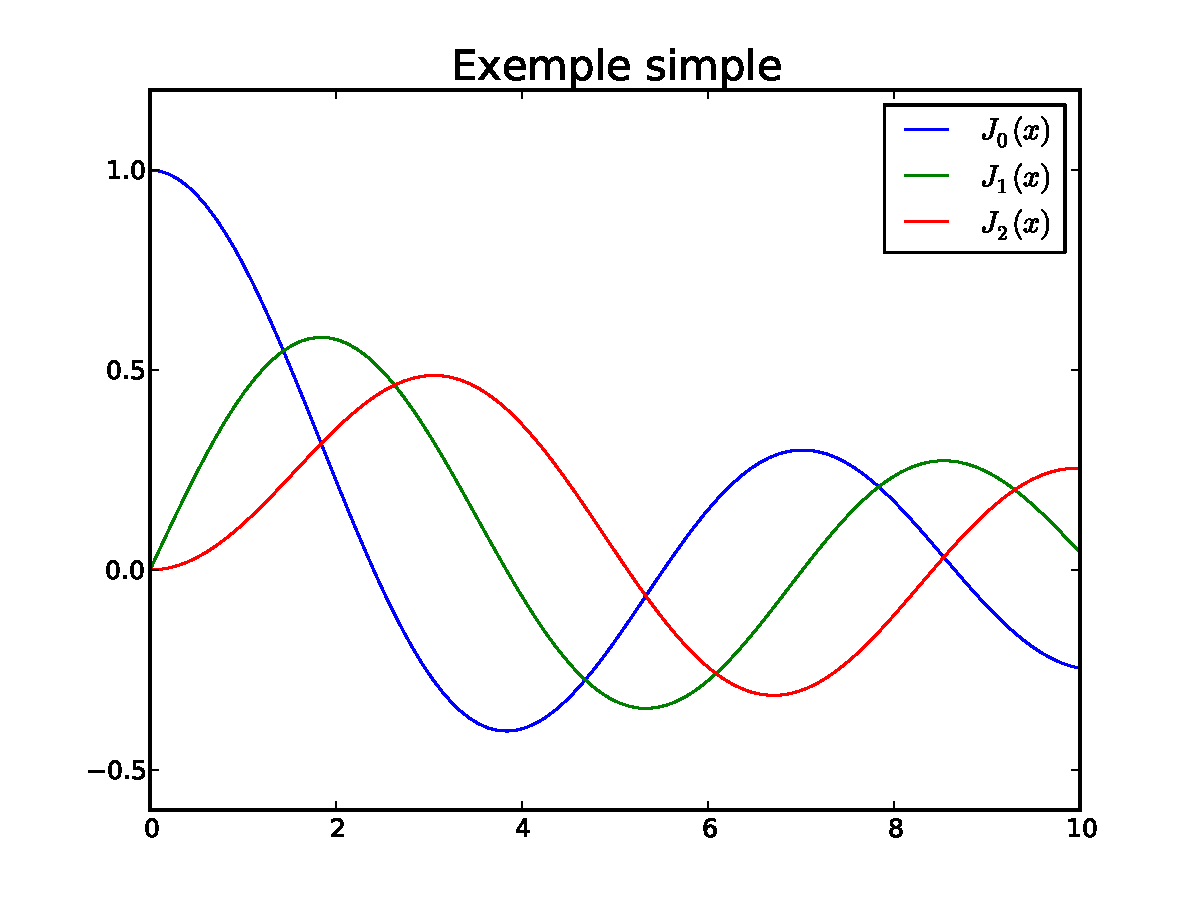
\includegraphics[clip,viewport=400 300 520 450,width=1.\textwidth]{example_simple_pdf}}
  \vspace{0.1cm}
  \centerline{(C) version .pdf}\medskip
\end{minipage}%
\caption{De pr\`es le .jpg c'est \textbf{VRAIMENT} nul. Vous pouvez zoomer sur la figure (C) pour bien voir l'intérêt d'un
format vectoriel}
\label{fig:ma_figure_zoom}
\end{figure}


\section{Liens hypertextes}

Pour ce faire il faut utiliser les packages pdftex et hyperref.
On insère un lien hypertexte par la commande 
\lstinline+\url+\nomenclature[A]{$\backslash$url}{$\backslash$url} si l'on veut écrire un lien 
hypertexte présentant le site cible. 
Par exemple on peut trouver de l'aide sur \LaTeX{} sur le site officiel : 
\url{http://www.ctan.org/} (la commande est \lstinline+\url{http://www.ctan.org/}+). 
Mais on peut aussi le faire avec  \lstinline+\href+, qui permet de définir n'importe quel mot 
comme lien. 
Par exemple \href{http://www.ctan.org/}{là} se trouve le site donné ci-dessus 
(avec la commande : \lstinline+\href{http://www.ctan.org/}{adresse}+).  
Les références, citations, entrées de la table des matières sont directement hypertextes 
(c.-à-d qu'on peut cliquer dessus pour aller à l'emplacement correspondant).
On pourra utiliser la ligne suivante pour définir divers packages utiles  d'un seul coup :
\begin{lstlisting}
\usepackage[pdftex,a4paper,linkcolor=test,citecolor=vertsombre,
	    colorlinks=true,pagebackref,bookmarks=true, 
	    plainpages=true,urlcolor=freeblue]{hyperref}
\end{lstlisting}

\section{Insérer un algorithme}
Plutôt que de donner un fichier de programmation, il peut être utile d'introduire dans son document
 un schéma de l'algorithme que l'on a utilisé. Pour cela, on peut choisir le package 
\lstinline+algpseudocode+

On peut alors obtenir  l'exemple suivant :\medskip 


\begin{algorithm}[h]
\KwData{les observations et leurs étiquettes $\mathcal{D}_n=\{(\mathbf{x}_i,y_i): 1\leq i \leq n\}$;
le pas de gradient: $\epsilon$; \qquad\qquad le nombre maximal d'it\'erations: $n_{\rm iter}$;}
\KwResult{$\mathbf{w}$}
initialiser (aléatoirement) $\mathbf{w}$ et  $j=0$\\
\While{$j\leq n_{\rm iter}$}{
$\mathbf{w}_{\rm{old}}\leftarrow\mathbf{w}$\\
\For{$i=1$ to $n$}{
$\mathbf{w}\leftarrow\mathbf{w}_{\rm{old}}-\epsilon 
\nabla_\mathbf{w}\ell( \hat{f}_{\mathbf{w}_{\rm{old}}}
(\mathbf x_i),y_i)$
}
$j\leftarrow j+1$
}
\caption{Perceptron}
\end{algorithm}

Les commandes utilisées sont: 

\begin{lstlisting}
\begin{algorithm}[h]
\KwData{Observations et \'etiquettes 
$\mathcal{D}_n=\{(\mathbf{x}_i,y_i): 1\leq i \leq n\}$;
le pas de gradient: $\epsilon$; \qquad\qquad 
le nombre maximal d'it\'erations: $n_{\rm iter}$;}
\KwResult{$\mathbf{w}$}
initialiser (al\'eatoirement) $\mathbf{w}$; initialiser  $j=0$\\
\While{$j\leq n_{\rm iter}$}{
$\mathbf{w}_{\rm{old}}\leftarrow\mathbf{w}$\\
\For{$i=1$ to $n$}{
$\mathbf{w}\leftarrow\mathbf{w}_{\rm{old}}-\epsilon 
\nabla_\mathbf{w}\ell( \hat{f}_{\mathbf{w}_{\rm{old}}}
(\mathbf x_i),y_i)$
}
$j\leftarrow j+1$
}
\caption{Perceptron}
\end{algorithm}
\end{lstlisting}

%% ATTENTION probl\`eme d'accent possible dans l'envuironnement lstlisting

\noindent Pour plus de détail sur ce package :

\noindent\url{www.ctan.org/get/macros/latex/contrib/algorithmicx/algorithmicx.pdf}

\section{Insertion de R et Python en \LaTeX{} }
Il est de plus en plus aisé d'écrire un rapport qui produit des graphiques (ou d'autres sorties, conclusions,etc.)
qui se base sur un langage. 

Un exemple simple est le cas d'une personne qui doit refaire toute les semaines un rapport presque identique,
sur une certaine base de données (CAC40, mesures de laboratoires ou autre) qui evolue au cours du temps.
Pour generer automatiquement un fichier synthetisant l'evolution, il peut etre bon d'utiliser des scriptes dans
son langage favori, et de faire en sorte que le pdf appelle en fait ces scriptes.
Cela peut se faire sous R et sous Python de la facon suivante:
on creer un fichier avec du latex qui produira le fichier pdf final, et on lance des scriptes de divers langages
pour produire les sorties graphiques, tableaux, etc.



Pour cela on peut utiliser \href{leisch.userweb.mwn.de/Sweave/}{Sweave} et 
\href{http://mpastell.com/pweave/}{Pweave} respectivement pour  R et python. Voir par exemple le 
\href{http://www.johndcook.com/blog/2012/12/20/basics-of-sweave-and-pweave/}{blog de John D. Cook},
pour plus details.



\section{Moosetex}

Pour les utilisateurs de Linux et Mac on pourra utiliser 
\href{http://www.math.u-bordeaux1.fr/~cdeledal/moosetex}{Moosetex},
principalement pour la gestion de l'insertion des images.
Un plus pour la fonction de nettoyage (moosetex cleaning) \`a utiliser par exemple
avant de faire une mise \`a jour sur un système de versionnement type git ou svn.
\mytodo{Charles petit laius?}